%%%%%%%%%%%%%%%%%%%%%%%%%%%%%%%%%%%%%%%%%%%%%%%%%%%%%%%%%%%%%%%%%%%%%%%%%%%%%%%
%%%%%%%%%%%%%%%%%%%%%%%%%%%%%%%%%%%%%%%%%%%%%%%%%%%%%%%%%%%%%%%%%%%%%%%%%%%%%%%
\chapter{Introduction}
\label{chap:introduction}
%%%%%%%%%%%%%%%%%%%%%%%%%%%%%%%%%%%%%%%%%%%%%%%%%%%%%%%%%%%%%%%%%%%%%%%%%%%%%%%
%%%%%%%%%%%%%%%%%%%%%%%%%%%%%%%%%%%%%%%%%%%%%%%%%%%%%%%%%%%%%%%%%%%%%%%%%%%%%%%

\begin{markdown}
-   Formalized score control
-   Research into same
-   This is a treatise
\end{markdown}

%%%%%%%%%%%%%%%%%%%%%%%%%%%%%%%%%%%%%%%%%%%%%%%%%%%%%%%%%%%%%%%%%%%%%%%%%%%%%%%
\section{Personal Background}
%%%%%%%%%%%%%%%%%%%%%%%%%%%%%%%%%%%%%%%%%%%%%%%%%%%%%%%%%%%%%%%%%%%%%%%%%%%%%%%

\begin{markdown}
-   khml
    -   An early example of maquette
-   nptl_b
    -   Max to spreadsheets, then by hand
    -   Notion of parametric specification
-   mbrsi
    -   Max to spreadsheets, then by hand
    -   Notion of timespans already established
    -   Incredibly labor intensive
    -   Attempted to automate via Illustrator, failed
    -   One single fabric, unfolding
    -   Impossible to maquette different textures together
-   aurora
    -   Revived the project, years later
    -   Implemented entirely in Python with Abjad
    -   Rendered by LilyPond
    -   Finally possible to maquette textures
    -   No time-signature changes possible: as though on flat grid
-   plague water
    -   Time signatures!
-   invisible cities
    -   Modernized the work done in plague water
\end{markdown}

%%%%%%%%%%%%%%%%%%%%%%%%%%%%%%%%%%%%%%%%%%%%%%%%%%%%%%%%%%%%%%%%%%%%%%%%%%%%%%%
\section{Historical Background}
%%%%%%%%%%%%%%%%%%%%%%%%%%%%%%%%%%%%%%%%%%%%%%%%%%%%%%%%%%%%%%%%%%%%%%%%%%%%%%%

\begin{markdown}
-   Patchwork
-   OpenMusic
-   PWGL
-   Bach
-   SuperCollider
-   Score
-   Rhinoceros and Grasshopper
-   Why didn't I use any of these?
    -   I realized text-based work was the right way to go
    -   Rapid prototyping, legibility, visualization all important
    -   Need a well-maintained language
\end{markdown}

%%%%%%%%%%%%%%%%%%%%%%%%%%%%%%%%%%%%%%%%%%%%%%%%%%%%%%%%%%%%%%%%%%%%%%%%%%%%%%%
\section{\emph{Mise-en-place}: composing at the command-line}
%%%%%%%%%%%%%%%%%%%%%%%%%%%%%%%%%%%%%%%%%%%%%%%%%%%%%%%%%%%%%%%%%%%%%%%%%%%%%%%

\begin{markdown}
-   Who is this for?
-   Why am I writing this?
-   What is this really about?
\end{markdown}

\subsection{Python}

\begin{singlespacing}
\vspace{-0.5\baselineskip}
\begin{lstlisting}
workstation:~ josiah\$ python
Python 2.7.8 (v2.7.8:ee879c0ffa11, Jun 29 2014, 21:07:35)
[GCC 4.2.1 (Apple Inc. build 5666) (dot 3)] on darwin
Type "help", "copyright", "credits" or "license" for more information.
>>>
\end{lstlisting}
\end{singlespacing}

\begin{comment}
<abjad>
1 + 1
</abjad>
\end{comment}

\begin{abjadbookoutput}
\begin{singlespacing}
\vspace{-0.5\baselineskip}
\begin{lstlisting}
>>> 1 + 1
2
\end{lstlisting}
\end{singlespacing}
\end{abjadbookoutput}

\subsection{LilyPond}

foo

\begin{singlespacing}
\vspace{-0.5\baselineskip}
\begin{multicols}{2}
\lstinputlisting[language=]{assets/example-es-ist-genug.ly}
\vfill
\columnbreak
\setlength\fboxsep{0pt}
\setlength\fboxrule{0.5pt}
\noindent\fbox{
    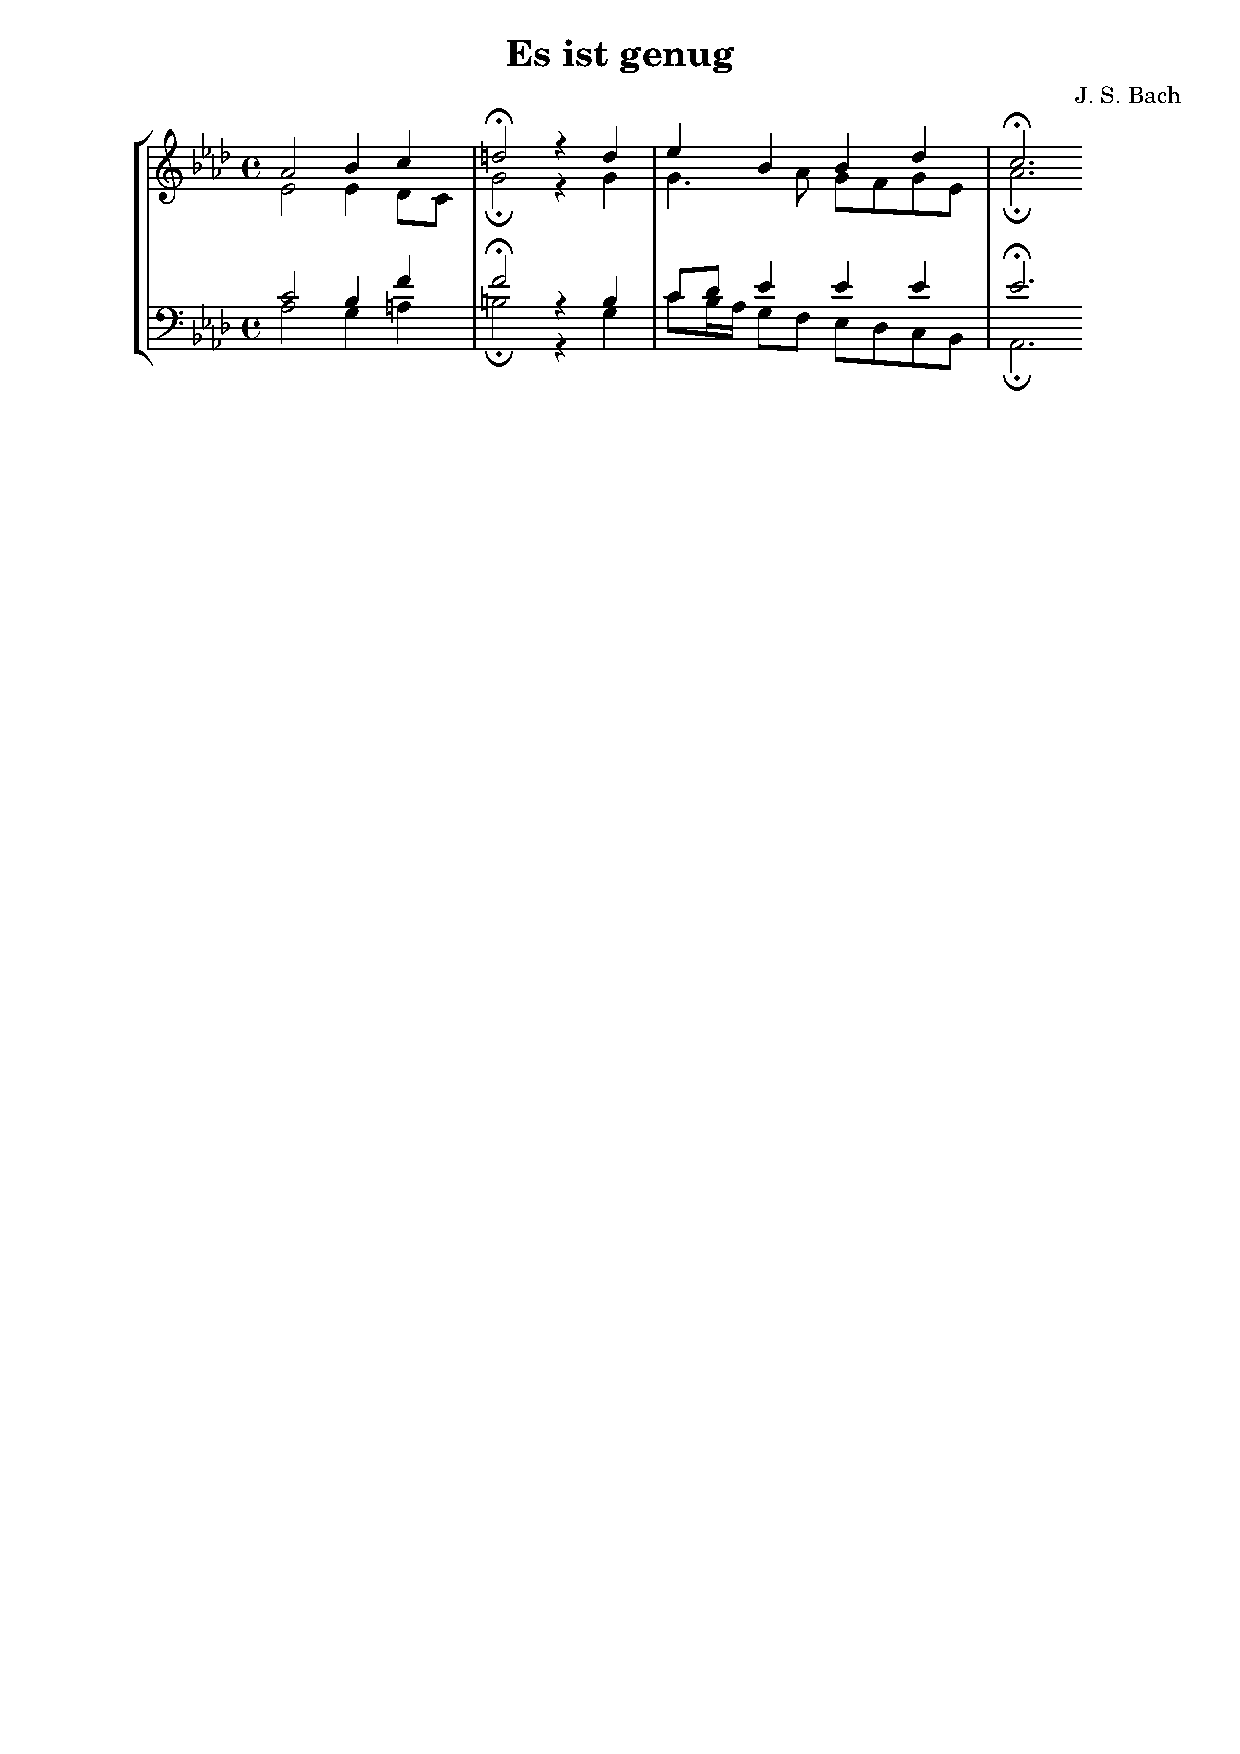
\includegraphics[scale=0.3875]{assets/example-es-ist-genug.pdf}
}
\end{multicols}
\end{singlespacing}

foo

\subsection{LaTeX}

foo

\begin{singlespacing}
\vspace{-0.5\baselineskip}
\begin{multicols}{2}
\lstinputlisting[style=beep]{assets/example-document.tex}
\vfill
\columnbreak
\setlength\fboxsep{0pt}
\setlength\fboxrule{0.5pt}
\noindent\fbox{
    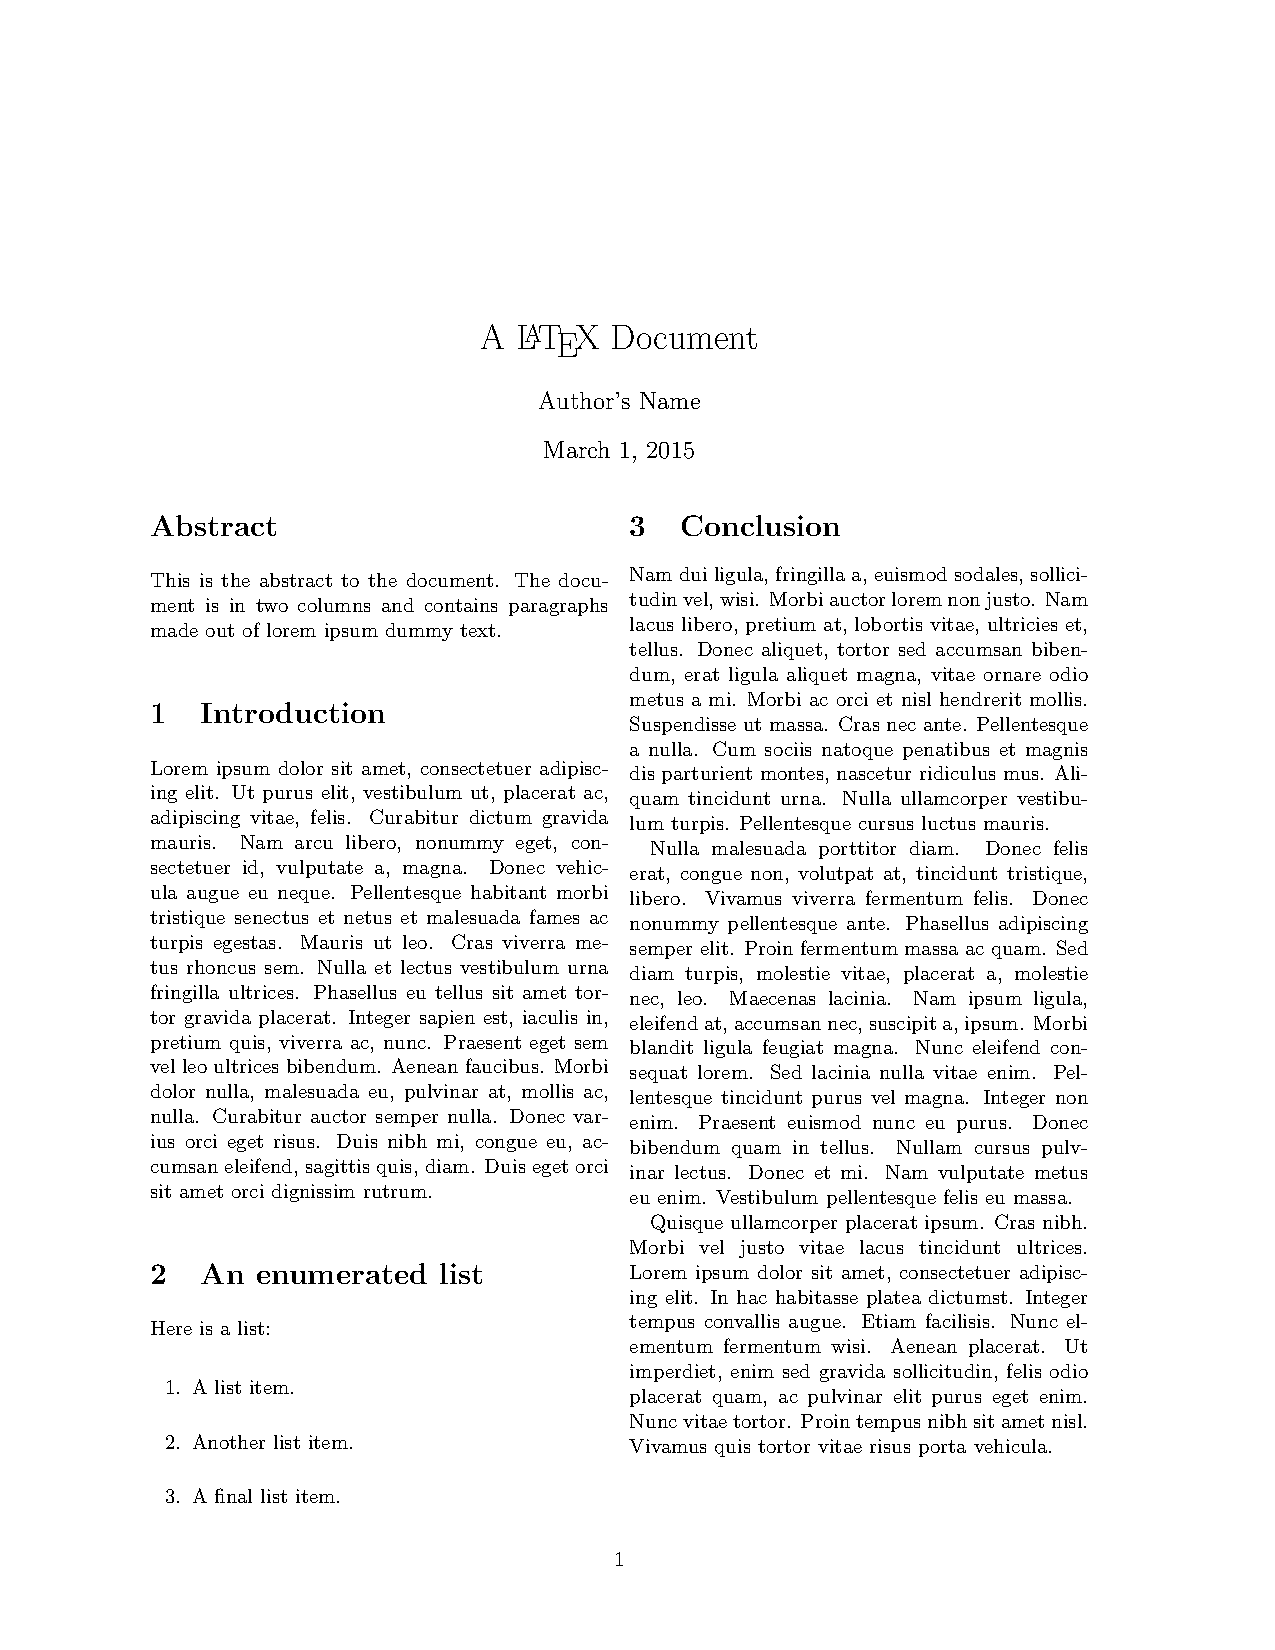
\includegraphics[scale=0.3875]{assets/example-document.pdf}
}
\end{multicols}
\end{singlespacing}

\subsection{Abjad}

foo

\subsection{Consort}

foo